
Fast- Slow systems are systems of differential equations that can be viewed on two different time scales, which are separated by a parameter.
These systems are generally of the form
\begin{align} 
\begin{cases}
x' &=\frac{dx}{dt}= f(x,y,\lambda, \epsilon),\\
y' &= \frac{dy}{dt}= \epsilon g( x,y, \lambda, \epsilon),
\end{cases}\label{FastS}
\end{align}
which is known as the fast system.
Using a scaling for the time, $t = \frac{\tau}{\epsilon} $, we find that this can be rewritten as
\begin{align}
\begin{cases}
\epsilon \dot{x} &= \epsilon \frac{dx}{d \tau} = f(x,y,\lambda, \epsilon),\\
\dot{y} & = \frac{dy}{d \tau} =  g( x,y, \lambda, \epsilon),
\end{cases}\label{SlowS}
\end{align}
which is called the slow system.\\

Here $x$ is called the fast variable, while $y$ is the slow variable. $\lambda$ is a parameter (see Section \ref{sec:canard-points}), $\epsilon$ is the time scale separation parameter and satisfies $0< \epsilon << 1$. The functions $f$ and $g$ are required to be sufficiently smooth \st we have $ C^{r+1} $ smoothness, where $ r $ is the number of dimensions present. It is generally possible to have three or more time scales, separated by additional parameters, as well as more state-space variables. \\

In order to analyse systems (\ref{FastS}) and (\ref{SlowS}) using Geometric Singular Pertubation Theory (GSPT), the singular limit $\epsilon \to 0$ is considered:

\begin{align} \label{FastS0}
\begin{cases}
x' &=\frac{dx}{dt}= f(x,y,\lambda, \epsilon)\\
y' &= 0,
\end{cases}
\end{align}
which is called the layer problem, and
\begin{align}\label{SlowS0}
\begin{cases}
0 &= \epsilon \frac{dx}{d \tau} = f(x,y,\lambda, 0)\\
\dot{y} & = \frac{dy}{d \tau} =  g( x,y, \lambda,0),
\end{cases}
\end{align}
called the reduced system.\\

Now considering Equation \ref{SlowS0}, we can write $f(x,y,\lambda, 0)=0$. Then we are able to define the critical manifold as:,
\begin{align} \label{CriticalS}
S= \left\{ (x,y) : f(x,y,\lambda, 0)=0 \right \},
\end{align}
where, by definition of $S$, the points $(x,y) \in S$ are equilibria of (\ref{FastS0}). Before we continue, it is useful to have a visual interpretation of these flows, 
\begin{figure}[h!]\centering

	\begin{subfigure}[t]{0.45\textwidth}
		\centering
		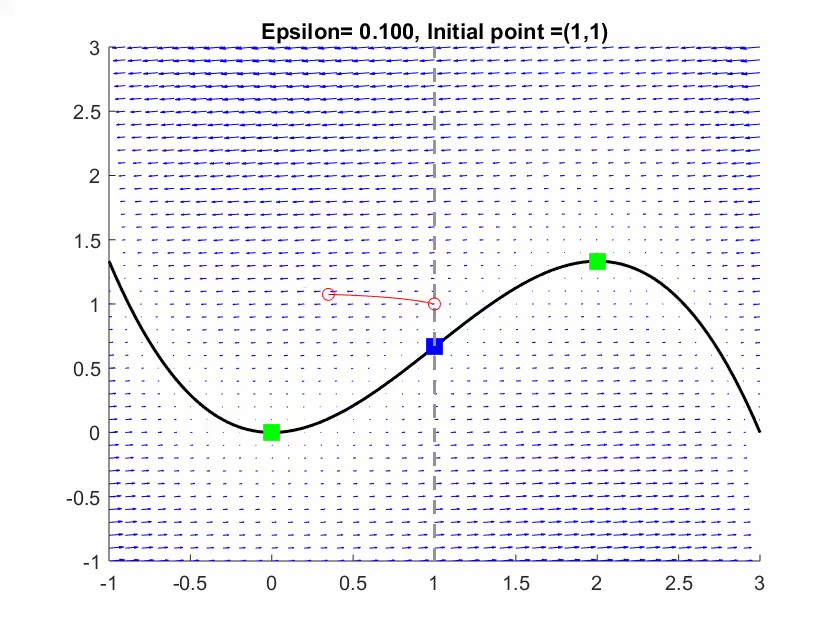
\includegraphics[width=.8\linewidth]{vdPhopf-Moment-1.jpg}
		\caption{The initial flow within the system starting at $ (x,y)=(1,1) $.} 
	\end{subfigure}
	\hfill
	\begin{subfigure}[t]{0.45\textwidth}
		\centering
		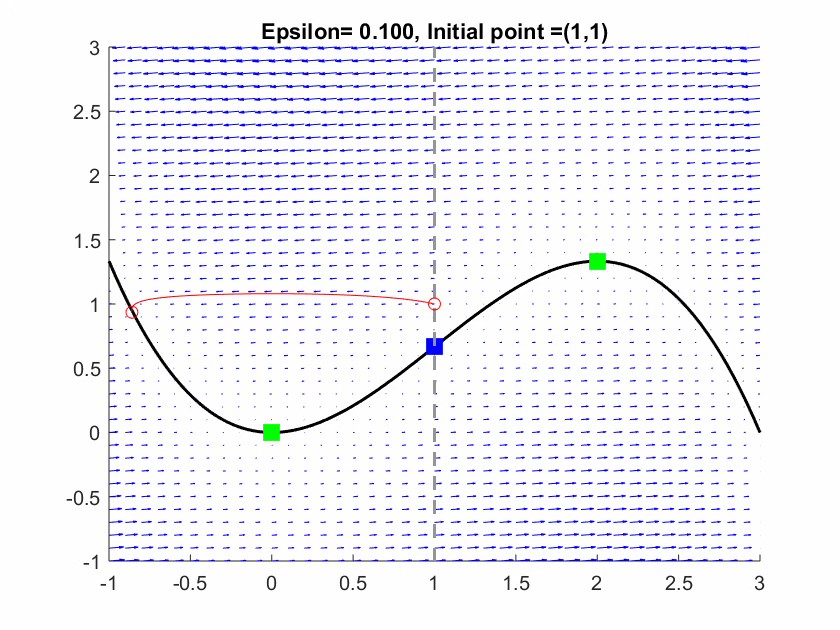
\includegraphics[width=.8\linewidth]{vdPhopf-Moment-2.jpg}
		\caption{The flow as it hits the slow manifold.} 
	\end{subfigure}
	
	\vspace{1cm}
	\begin{subfigure}[t]{0.45\textwidth}
		\centering
		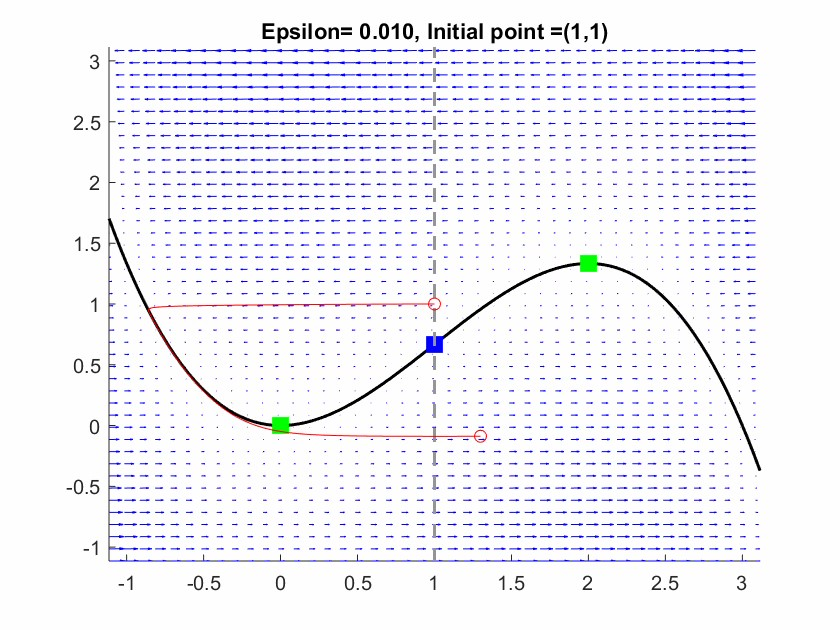
\includegraphics[width=.8\linewidth]{vdp-jump1}
		\caption{The flow as it intersects with the fold point and begins the jump.} 
	\end{subfigure}
	\hfill
	\begin{subfigure}[t]{0.45\textwidth}\centering
		% just an empty subfigure to shift C below A
		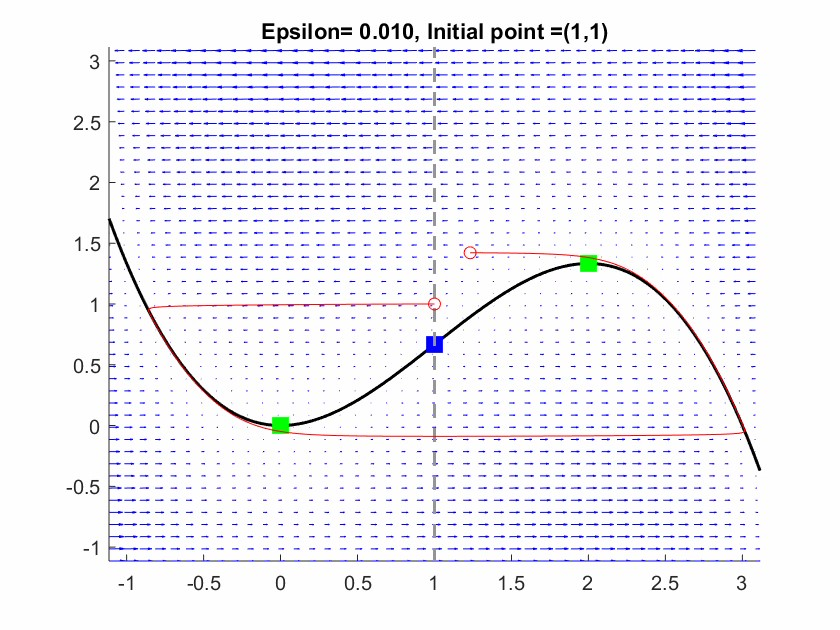
\includegraphics[width=.8\linewidth]{vdp-jump2}
		\caption{The second jump before continuing in a periodic fashion.}
	\end{subfigure}
	\caption{Flows in the \vdp system.}
	\label{fig: vdp flow diagram}
\end{figure}\newline
where we can see that the flows will travel towards our fold point, following the relevant branches. It is worth noting that our flow does not meet the fold point exactly, although this is an `error', it does not directly effect our simulations - as is discussed in Section \ref{sec:matlab-stuff}.


\section{Geometric Singular Pertubation Theory} \label{GSPT}

The main idea of GSPT is the following: Under certain conditions it can be concluded that the critical manifold $S=S_0$, where $\epsilon \to 0$ persists as an invariant manifold $S_{\epsilon}$ under a small pertubation $\epsilon >0$, if $\epsilon$ is sufficiently small. In higher than 2 dimensions the idea of transversality of the flow of the stable and unstable manifolds is essential for analysis, while in 2 dimensions this is rather trivial \citep{MMO}. The main contribution to GSPT comes from Fenichel Theory and his three Theorems can be summed up in one, according to \citep{MMO}.
However, before stating the Theorem, some formal definitions are needed.

\begin{definition}{\textbf{Normal Hyperbolicity \citep{firstpaper}}} \label{NormHyp}
	\\
	A submanifold $M \subseteq S$ is called normally hyperbolic, if the Jacobian $ \frac{\partial f}{\partial x}(x,y, \lambda, 0),$ where $(x,y) \in M$, has only eigenvalues with nonzero real part.
\end{definition} 

Moreover, the points $(x,y) \in M$, $M$ normally hyperbolic, are hyperbolic equilibria of Equation \ref{FastS0} \citep{MMO}.
A normally hyperbolic submanifold can be classified according to its stability property: If $M$ only has eigenvalues with positive real part it is called repelling, otherwise eigenvalues with negative real part are called attracting and if $M$ is neither attracting nor repelling it is called a saddle-type submanifold \citep{MMO}. \\

Furthermore, stable and unstable manifolds can be defined as $W^s(M)$  and $W^u(M)$, corresponding to the eigenvalues with negative and positive real part, respectively. Furthermore, with the following definition it is established which notion of distance is going to be employed throughout this analysis.

\begin{definition}{\textbf{Hausdorff Distance \citep{Kuehn}}}\\
	The Hausdorff Distance of two nonempty sets $V,W \subset \mathbf{R}^n$, for some $n \in \mathbf{N}$ 
	is defined as 
	\begin{align*}
	d_H(V,W)= \max \{ \sup_{v \in V} \inf_{w \in W} || v- w ||, \sup_ {w \in W}\inf_{v \in V} || v- w ||\}.
	\end{align*}
%	(ref: book kuehn)
\end{definition}

Now combining the above we can state Fenichel's Theorem.
\begin{theorem}{\textbf{Fenichel's Theorem}} \label{Fenichel}
	\\
	Suppose $M=M_0$ is a compact, normally hyperbolic submanifold  (possibly with boundary) of the critical manifold $S$ Equation \ref{CriticalS} and  that $f, g \in C^r, r < \infty $. Then for $\epsilon >0$, sufficiently small, the following holds:\\
	(F1) There exists a locally invariant manifold $M_{\epsilon}$, diffeomorphic to  $M_0$. Local invariance means that $M_{\epsilon}$ can have boundaries through which trajectories enter or leave.\\
	(F2) $M_{\epsilon}$ has a Hausdorff distance of $O(\epsilon)$ from $M_0$.\\
	(F3) The flow on $M_{\epsilon}$  converges to the slow flow as $\epsilon \to 0$.\\
	(F4) $M_{\epsilon}$ is $C^r$- smooth.\\
	(F5) $M_{\epsilon}$ is normally hyperbolic and has the same stability properties with respect to the fast variabes as $M_0$ (attracting, repelling or saddle type).\\
	(F6) $M_{\epsilon}$ is usually not unique. In regions that remain at a fixed distance from the boundary of  $M_{\epsilon}$, all manifolds satisfying (F1)-(F5) lie at a Hausdorff distance $O(e^{-K/\epsilon})$ from each other for some $K>0$ with $K=O(1)$.\\
	The normally hyperbolic manifold $M_0$ has associated local stable and unstable manifolds
	\begin{align*}
	W^s(M_0) =\cup_{p \in M_0} W^s(p) \textrm{\ \ and\ \ } W^u(M_0) =\cup_{p \in M_0} W^u(p),
	\end{align*}
	where  $W^s(p)$ and $W^u(p)$ are the local stable and unstable manifolds of $p$ as a hyperbolic equilibrium of the layer equations, respectively. These manifolds also persist for $\epsilon > 0$, sufficiently small: there exist locally stable and unstable manifolds $W^s(M_\epsilon)$ and $W^u(M_\epsilon)$, respectviely, for which conclusions (F1) - (F6) hold if we replace $M_\epsilon$ and $M_0$ by  $W^s(M_\epsilon)$ and $W^s(M_0)$ (or similarly by  $W^u(M_\epsilon)$ and $W^u(M_0)$).
\end{theorem} +++direct citation needed for theorem (MMO) +++

Fenichel's Theorem establishes that the submanifold, $M_0$, of the critical manifold, $S_0$, persists as slow manifold $M_\epsilon$ as $\epsilon >0$, given it is compact and normally hyperbolic. The theorem furthermore establishes that the stable and unstable manifolds persist as well as the individual fibres, namely $W^s(p)$ and $W^u(p)$, that are associated to each base point $p \in M_0$.
Therefore, under the assumptions of the theorem, the flow of the Fast-Slow system remains $O(\epsilon)$ close to the flow of the system in the singular limit $\epsilon \to 0$.\\

The importance of this result lies in the fact that the behaviour of the full system can be analysed by looking at the system in the singular limit instead, which is often more practical.


++++++++++++also trajectories can be constructed and tested using fenichel... paper 1++++++++++


